\documentclass[ignorenonframetext,xcolor=x11names]{beamer}

\definecolor{mun}{RGB}{134,38,51}
\definecolor{mun2}{RGB}{99,102,106}
%\definecolor{mun}{cmyk}{0,.3922,.2392,.1686}
\definecolor{code}{RGB}{0, 0, 128}
\definecolor{code}{gray}{0.95}

\mode<presentation>
{
%  \usetheme{boxes}
%  \usetheme{default}
%  \usetheme{Montpellier}
%  \usetheme{Singapore}
%   \usetheme{Rochester}
%  \usecolortheme{crane}
%  \usecolortheme{dolphin}
%  \usecolortheme{lily}
%  \usecolortheme{orchid}
  \usecolortheme{rose}
  \setbeamercovered{transparent}
%  \usefonttheme[onlymath]{serif}
  \setbeamercolor*{structure}{bg=mun,fg=mun}
  \setbeamercolor*{palette primary}{use=structure,fg=white,bg=structure.fg}
  \setbeamercolor*{palette secondary}{use=structure,fg=white,bg=structure.fg}
  \setbeamercolor*{palette tertiary}{use=structure,fg=white,bg=black}
  \setbeamercolor*{palette quaternary}{fg=white,bg=black}
  \setbeamercolor{section in toc}{fg=black,bg=white}
  \setbeamercolor{alerted text}{use=structure,fg=structure.fg!50!black!80!black}
  \setbeamercolor{titlelike}{parent=palette primary,fg=structure.fg!50!black}
  \setbeamercolor{frametitle}{bg=mun,fg=white}
  \setbeamercolor*{titlelike}{parent=palette primary}

  \setbeamercolor{normal text}{fg=black!90}
  \setbeamercolor{math text}{fg=black}
  \setbeamercolor{quote}{bg=gray!20}
  \setbeamercolor{quotation}{bg=gray!20}
  \setbeamerfont{cite}{size=\scriptsize}
  \setbeamerfont{quote}{size=\footnotesize}
  \setbeamerfont{quotation}{size=\footnotesize}
  \setbeamercolor{red text}{fg=red!75!black}
  \setbeamertemplate{bibliography item}[triangle]
  \setbeamertemplate{enumerate item}[square]
  \setbeamertemplate{blocks}[rounded][shadow=true]
  \setbeamertemplate{navigation symbols}{}
  \setbeamertemplate{footline}[frame number]
}
\usepackage{tcolorbox}
\usepackage{amsmath}
\usepackage{physics}
\usepackage{pgf}
\usepackage[english]{babel}
\usepackage[latin1]{inputenc}
\usepackage{times}
\usepackage[T1]{fontenc}
\usepackage{multicol}
\usepackage{multirow}
\usepackage{fancyvrb}
\usepackage{tabularx}
\usepackage{amsmath}
\usepackage{bbm}
\usepackage{alltt}
\usepackage{hyperref}
\hypersetup{
    colorlinks=true,
    linkcolor=blue,
    filecolor=magenta,      
    urlcolor=blue,
}
\usepackage{minted}
\newminted{cypher}{autogobble,bgcolor=code,breakbytoken,frame=single,framesep=3pt}
\newminted{R}{autogobble,bgcolor=code,breakbytoken,frame=single,framesep=3pt}
\newminted{text}{autogobble,bgcolor=code,breakbytoken,frame=single,framesep=3pt}
\newminted{sql}{autogobble,bgcolor=code,breakbytoken,frame=single,framesep=3pt}
\newminted{bash}{autogobble,bgcolor=code,breakbytoken,python3,frame=single,framesep=3pt}
\newminted{xml}{autogobble,bgcolor=code,breakbytoken,python3,frame=single,framesep=3pt}
\newminted{python}{bgcolor=code,breakbytoken,python3,frame=single,framesep=3pt}
\newminted{html}{autogobble,bgcolor=code,breakbytoken,frame=single,framesep=3pt}
\newminted{js}{autogobble,bgcolor=code,breakbytoken,frame=single,framesep=3pt}
\AtBeginEnvironment{minted}{%
  \renewcommand{\fcolorbox}[4][]{#4} \scriptsize}
\AtEndEnvironment{minted}{%
  \normalsize}

%\newcommand{\Pr}{\operatorname{Pr}}
\newcommand{\argmax}{\operatorname*{argmax}}
\newcommand{\argmin}{\operatorname*{argmin}}
\newcommand{\Ident}{\operatorname{I}}

\author % (optional, use only with lots of authors)
{Joerg Evermann}
% - Give the names in the same order as the appear in the paper.
% - Use the \inst{?} command only if the authors have different
%   affiliation.

\institute%[Universities of Somewhere and Elsewhere] % (optional, but mostly needed)
{
  Faculty of Business Administration\\
  Memorial University of Newfoundland \\ 
  \texttt{jevermann@mun.ca} 
}

\date{}

\pgfdeclareimage[width=1.5cm]{university-logo}{../MUN_LOGO_CMYK}
\logo{\pgfuseimage{university-logo}}

% If you wish to uncover everything in a step-wise fashion, uncomment
% the following command: 

%\beamerdefaultoverlayspecification{<+->}

 
\title{Business 4720 - Class 6}

\subtitle{Data Management in Python using Pandas}

\begin{document}

\begin{frame}{}
  \titlepage
  \footnotesize
  \begin{center}

\includegraphics[height=.5in]{../by-nc.png}

Unless otherwise indicated, the copyright in this material is owned by Joerg Evermann. This material is licensed to you under the \href{https://creativecommons.org/licenses/by-nc/4.0/}{Creative Commons by-attribution non-commercial license (CC BY-NC 4.0)}
\end{center}

\end{frame}

\section{Introduction}

\begin{frame}{This Class}

\begin{block}{What You Will Learn:}
\begin{itemize}
  \item Introduction to Python
  \item Introduction to the the Numpy package
  \item Introduction to the Pandas package
\end{itemize}
\end{block}
\end{frame}

\section{R}

\begin{frame}{Intro to Python}
\begin{block}{What is Python?}
\begin{itemize}
    \item Readability and simplicity
    \item Dynamic typing enhancing flexibility
    \item Extensive libraries
    \item Procedural, object-oriented, and functional programming
    \item Widely used in data analysis, AI, scientific computing, etc.
    \item Easy to learn
    \item Active community support
\end{itemize}
\end{block}
\vspace{3mm}
\textbf{Intro Tutorial:} \\
\url{https://python.swaroopch.com/} \\
\url{https://github.com/swaroopch/byte-of-python/releases/}
\end{frame}


\begin{frame}{Running Python}
\begin{enumerate}
    \item Interactive Python Shell (command line)
    \item Jupyter Notebooks
    \item PyCharm IDE
\end{enumerate}
\end{frame}

\begin{frame}{Interactive Python Shell}
\begin{itemize}
    \item Similar to R
    \item Type ''python'' to launch Python interpreter
    \item Prompt is ''> > >'', type \colorbox{lightgray}{ENTER} to execute a command
    \item Use \texttt{quit()} to exit
    \item \textbf{Tip}: Use a notepad app to assemble commands and to keep results
\end{itemize}
\end{frame}

\begin{frame}{Interactive Python Shell}
\centering
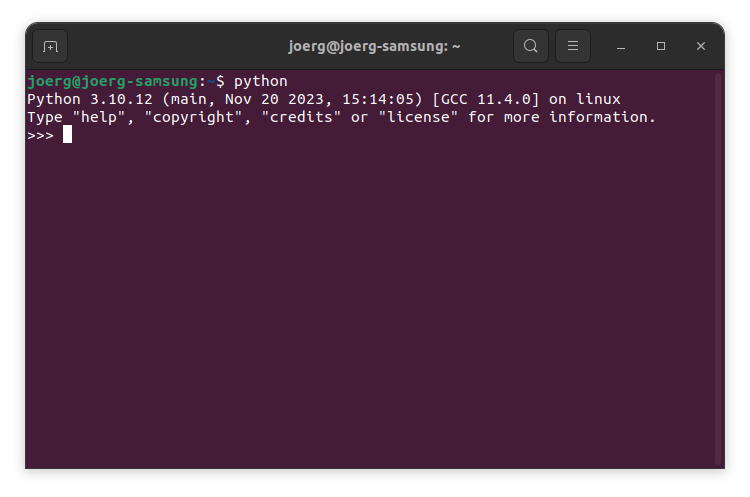
\includegraphics[width=\textwidth]{screen3.png}
\end{frame}

\begin{frame}{Jupyter Notebooks}
\begin{itemize}
    \item Interactive computing environment
    \item Notebook Interface
	\item Combine executable code, text, visualizations
	\item Create and share documents with live code, equations, and explanatory text
	\item Collaborative editing of notebooks (on web-based services)
	\item Popular for Python, but can handle other languages
\end{itemize}
\end{frame}

\begin{frame}{JupyterLabs Desktop}
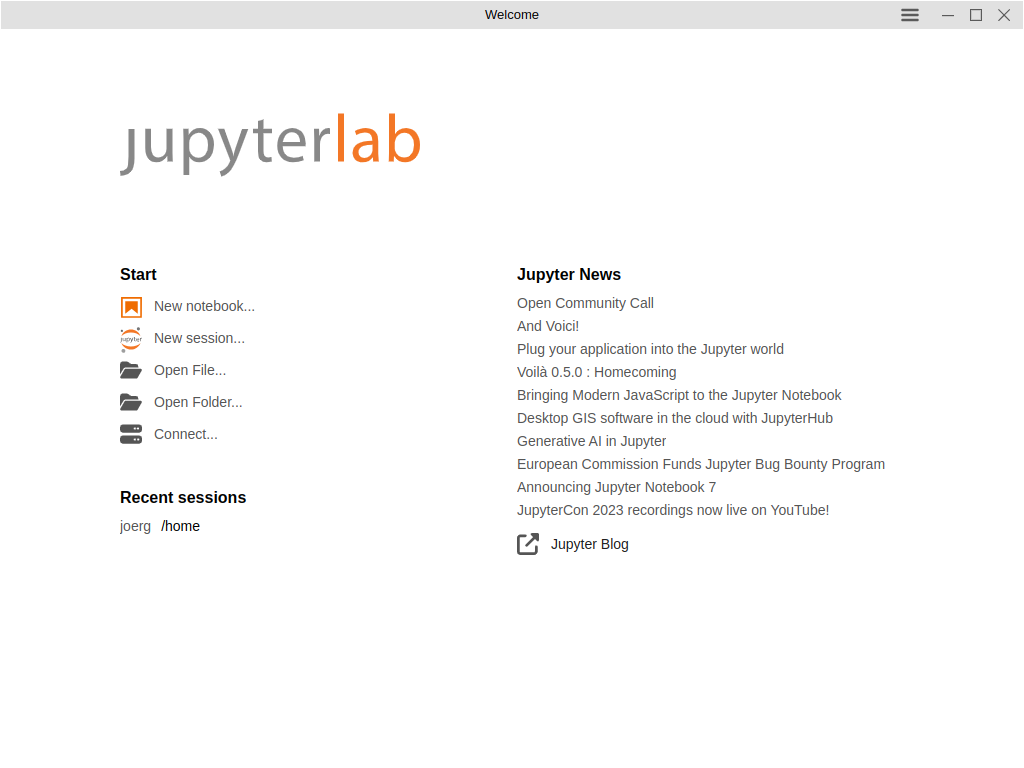
\includegraphics[width=\textwidth]{screen1.png}
\end{frame}

\begin{frame}{JupyterLabs Desktop}
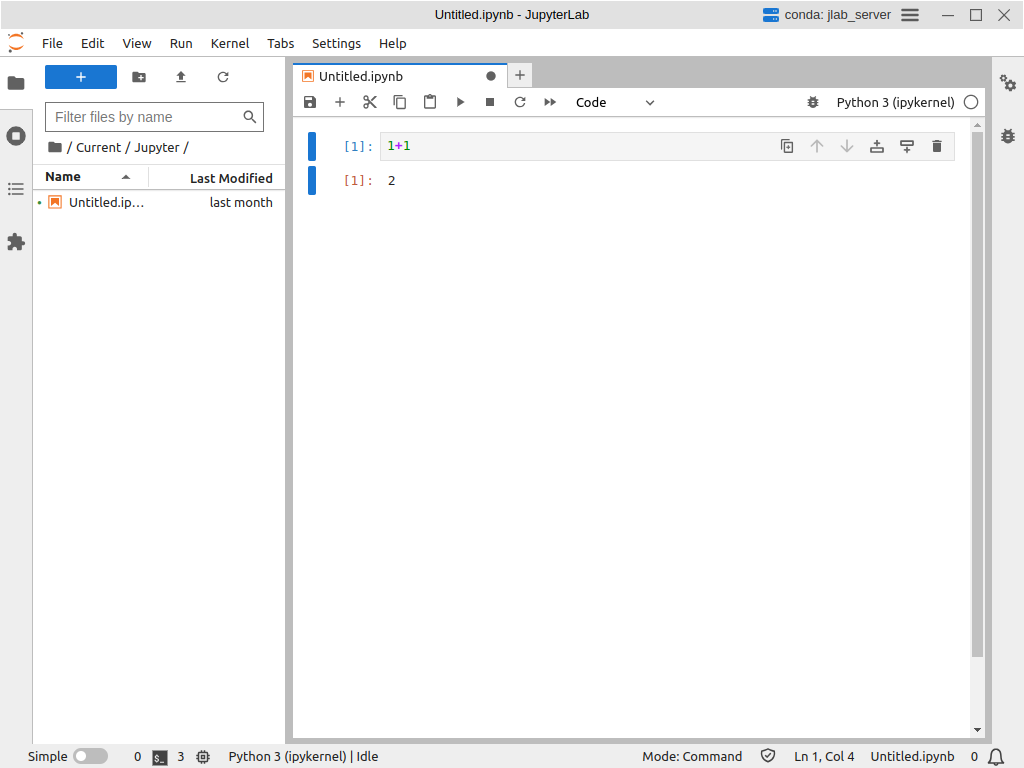
\includegraphics[width=\textwidth]{screen2.png}
\end{frame}

\begin{frame}{Jupyter Notebooks}
\begin{itemize}
  \item ''Kernel'' is the Python interpreter and environment that runs your code
  \item Enter code into empty cell
  \item Press \colorbox{lightgray}{CTRL-ENTER} to execute a cell
  \item Merge, split, move, copy, delete cells
  \item Save, import, export notebooks
\end{itemize}
\end{frame}

\begin{frame}{PyCharm IDE}
\begin{itemize}
   \item When working with multiple Python files in your project
   \item Useful for \emph{programming} (defining functions, classes; using control structures, etc.) rather than just \emph{scripting} (executing a few Python commands one after the other)
   \item Contains built-in debugging tools
\end{itemize}
\end{frame}

\begin{frame}{PyCharm IDE}
\centering
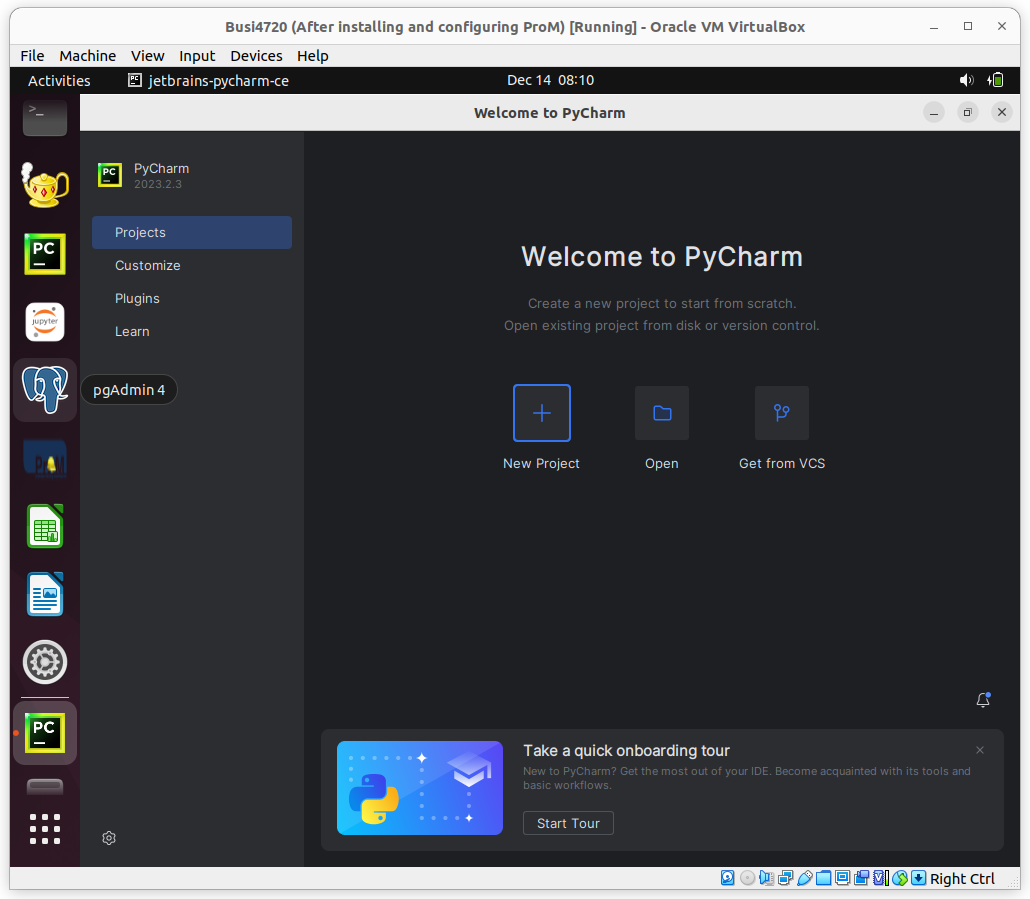
\includegraphics[height=2.5in]{screen4.png}
\end{frame}


\begin{frame}[fragile]{Basic Python}
Printing a string:
\footnotesize
\begin{pythoncode}
print('hello world')
\end{pythoncode}
\normalsize
String format method:
\footnotesize
\begin{pythoncode}
age = 19
name = 'Malina'
print('{0} is {1} years old'.format(name, age))
print('{name} is {age} years old'.format(name=name,age=age))
print('{} is {} years old'.format(name, age))
print(f'{name} is {age} years old')
print(name+' is '+str(age)+' years old')
\end{pythoncode}
\end{frame}

\begin{frame}[fragile]{Basic Python}
Backslashes split and continue lines:
\footnotesize
\begin{pythoncode}
print('This is a very long \
string and needs a second line')
i = \
5
print(i)
\end{pythoncode}
\normalsize
Multiline strings:
\footnotesize
\begin{pythoncode}
s = '''This is line 1
and here is line 2
and now this is line 3'''
print(s)
\end{pythoncode}
\normalsize
\end{frame}

\begin{frame}[fragile]{Basic Python}
Python knows math:
\footnotesize
\begin{pythoncode}
2 + 2
2**4
13 // 3
-13 // 3
13 % 3
-25.5 % 2.25
3 < 5
3 > 5
3 == 5
(3 < 5) and (4 < 2)
(3 < 5) or not (4 < 2)
\end{pythoncode}
\end{frame}

\begin{frame}[fragile]{Strings}
Python knows strings:
\footnotesize
\begin{pythoncode}
language = 'Innuktitut'
if language.startswith('Innu'):
    print('Yes, the string starts with "Innu"')
if 'u' in language:
    print('Yes, it contains the string "u"')
if language.find('nuk') != -1:
    print('Yes, it contains the string "nuk"')

# Joining and Splitting    
delimiter = '_*_'
mylist = ['Nain', 'Hopedale', 'Makkovik', 'Rigolet']
mystring = delimiter.join(mylist)
print(mystring)
thelist = mystring.split(delimiter)
print(thelist)
\end{pythoncode}
\end{frame}

\begin{frame}[fragile]{Lists}
Lists are ordered collections of items:
\footnotesize
\begin{pythoncode}
# Inuit deities
gods = ['Sedna', 'Nanook', 'Akna', 'Pinga']
print('There are', len(gods), 'deities:')
for item in gods:
    print(item, end=' ')

gods.append('Amaguq')
print('\nThe list of deities is now', gods)

gods.sort()
print('The sorted list is', gods)

print('The first deity is', gods[0])
olditem = gods[0]
del gods[0]
print('I removed', olditem)
print('The list is now', gods)
\end{pythoncode}
\end{frame}

\begin{frame}[fragile]{Tuples}
Tuples are immutable:
\footnotesize
\begin{pythoncode}
# Inuit Nunangat
regions = ('Inuvialuit', 'Nunavut', \
           'Nunavik', 'Nunatsiavut')
print('Number of regions is', len(regions))

all_regions = 'NunatuKavummiut', 'Kalaallit', \
              'Inupiaq', regions
print('Number of all Inuit regions:',len(all_regions))
print('All Inuit regions are', all_regions)
print('Regions in Inuit Nunangat are', all_regions[3])
print('First region in Inuit Nunangat is', \
      all_regions[3][1])
print('Number of all Inuit regions is', \
      len(all_regions)-1+len(all_regions[3]))
\end{pythoncode}
\end{frame}

\begin{frame}[fragile]{Dictionaries}
\begin{itemize}
  \item Key--value pairs
  \item Associative arrays
  \item Map
\end{itemize}
\scriptsize
\begin{pythoncode}
# Largest citites
c = {
    'Inuvialuit': 'Inuvik',
    'Nunavut': 'Iqaluit',
    'Nunavik': 'Kuujjuaq',
    'Nunatsiavut': 'Nain' 
}
print(c.keys())
print(c.values())

print("Nunavik's largest city is", c['Nunavik'])
# Deleting a key-value pair
del c['Nunavut']
print('\nThere are {} cities left\n'.format(len(c)))
for region, city in c.items():
    print('{} is largest city of {}'.format(city, region))
# Adding a key-value pair
c['Nunavut'] = 'Iqaluit'
if 'Nunavut' in c:
    print("\nNunavut's largest city is", c['Nunavut'])
\end{pythoncode}
\end{frame}

\begin{frame}{Structured Data Types}
\begin{block}{Important}
\begin{itemize}
  \item Indexing begins at 0 (different from R!)
  \item Can contain any data type
\end{itemize}
\end{block}

\begin{block}{Sequences}
\begin{itemize}
  \item List, tuples, strings are sequences
  \item Membership tests using \texttt{in} or \texttt{not in}
  \item Indexing and slicing
\end{itemize}
\end{block}
\end{frame}

\begin{frame}[fragile]{Slicing}
\footnotesize
\begin{pythoncode}
regions = ('Inuvialuit', 'Nunavut', 
           'Nunavik', 'Nunatsiavut')
language = 'Innuktitut'

# Slicing on a tuple
print('Item 1 to 3 is', regions[1:3])
print('Item 2 to end is', regions[2:])
print('Item 1 to -1 is', regions[1:-1])
print('Item start to end is', regions[:])
# Slicing on a string 
print('characters 1 to 3 is', language[1:3])
print('characters 2 to end is', language[2:])
print('characters 1 to -1 is', language[1:-1])
print('characters start to end is', language[:])
# Slicing with step
print(regions[::1])
print(regions[::2])
print(regions[::3])
print(regions[::-1])
\end{pythoncode}
\end{frame}

\begin{frame}{Hands-On Exercises}
\begin{block}{Lists}
\begin{enumerate}
    \item Create a list containing the numbers 1 to 10. Use list slicing to create a sublist with only the even numbers.
    \item Using a \texttt{for} loop, sum all the items in the list.
    \item Using a \texttt{for} loop, iterate over the list and print each number squared.
    \item Write a program to append the square of each number in the range [1:5] to a new list.
\end{enumerate}
\end{block}
\end{frame}
\begin{frame}{Hands-On Exercises}
\begin{block}{Tuples}
\begin{enumerate}
    \item Create a tuple with different data types (string, int, float).
    \item Demonstrate how tuples are immutable by attempting to change its first element.
    \item Write a program to convert the tuple into a list.
\end{enumerate}
\end{block}
\end{frame}
\begin{frame}{Hands-On Exercises}
\begin{block}{Dictionaries}
\begin{enumerate}
    \item Create a dictionary with at least three key-value pairs, where the keys are strings and the values are numbers.
    \item Write a Python script to add a new key-value pair to the dictionary and then print the updated dictionary.
    \item Create a nested dictionary and demonstrate accessing elements at various levels.
\end{enumerate}
\end{block}
\end{frame}

\begin{frame}{Numerical Data in Python with NumPy}
\begin{block}{What is Numpy?}
\begin{itemize}
    \item High-performance scientific computing and data analysis.    
    \item Multidimensional arrays
    \item Comprehensive mathematical function library
    \item Foundational package for other scientific libraries like SciPy, Pandas, Matplotlib, scikit-learn, scikit-image, etc.
\end{itemize}
\end{block}
\vspace{5mm}
\textbf{Intro Tutorials}: \\

\url{https://numpy.org/doc/stable/user/quickstart.html} \\
\url{https://numpy.org/doc/stable/user/absolute_beginners.html}
\end{frame}

\begin{frame}{NumPy Array}
N-Dimensional Array, type ''\texttt{ndarray}'' \\

\renewcommand{\arraystretch}{1.5}
\centering

\footnotesize
\begin{tabularx}{\linewidth}{l|X} \hline
\texttt{ndarray.ndim} & Number of axes \\
\texttt{ndarray.shape} & Typle describing the size of each dimension (axis) \\
\texttt{ndarray.size} & Total number of elements \\
\texttt{ndarray.dtype} & The datatype of the elements, e.g. \texttt{numpy.int32}, \texttt{numpy.int16}, \texttt{numpy.float32}, \texttt{numpy.float64} \\
\texttt{ndarray.itemsize} & Number of bytes for each element \\ \hline
\end{tabularx}
\end{frame}

\begin{frame}[fragile]{NumPy Basics}
\footnotesize
\begin{pythoncode}
# Import the numpy package
import numpy as np

# Create an array
a = np.arange(15).reshape(3, 5)
print(a.shape)
print(a.ndim)
print(a.dtype.name)
print(a.size)
print(type(a))
\end{pythoncode}
\end{frame}

\begin{frame}[fragile]{NumPy Basics}
\footnotesize
\begin{pythoncode}
# Create an array from Python lists and tuples
b = np.array([(1.5, 2., 3), (4, 5, 6)])
print(b)

# Elementwise operations
print(3 * b)
print(b + 5)
print(np.sqrt(b))

# Array operations
print(np.max(b))
print(np.max(b, axis=0))
print(np.max(b, axis=1))
print(np.std(b))
print(np.cov(b))
print(np.sum(b))
\end{pythoncode}
\end{frame}

\begin{frame}[fragile]{NumPy Basics \small [cont'd]}
\footnotesize
\begin{pythoncode}
# Create an array of zeros with shape (3,4)
x = np.zeros((3,4))
print(x)

# Create an array of ones with shape (2,3,4)
y = np.ones((2,3,4))
print(y)
\end{pythoncode}
\end{frame}

\begin{frame}[fragile]{Array Slicing}
\begin{itemize}
    \item Each axis can be sliced using \texttt{[:]} or \texttt{[::]}
\end{itemize}
\footnotesize
\begin{pythoncode}
b = np.array([[ 0,  1,  2,  3],
              [10, 11, 12, 13],
              [20, 21, 22, 23],
              [30, 31, 32, 33],
              [40, 41, 42, 43]])
              
print(b[2, 3])
print(b[0:5, 1])
print(b[:, 1])
print(b[1:3, :])
print(b[-1])
\end{pythoncode}
\end{frame}

\begin{frame}[fragile]{Array Slicing \& Iterators}
\footnotesize
\begin{pythoncode}
c = np.array([[[  0,  1,  2],
               [ 10, 12, 13]],
              [[100, 101, 102],
               [110, 112, 113]]])
               
print(c.shape)
print(c[1, ...])
print(c[1, : , : ])
print(c[..., 2])
print(c[: , : , 2])
print(c[..., : , 1])

for row in b:
    print(row)
    
for element in b.flat:
    print(element)
\end{pythoncode}
\end{frame}

\begin{frame}[fragile]{Array Reshaping}
\footnotesize
\begin{pythoncode}
rg = np.random.default_rng(1)
a = np.floor(10 * rg.random((3, 4)))

print(a.shape)
print(a.flatten())
print(a.reshape(6, 2))
print(a.T)
print(a.T.shape)

b = np.floor(5 * rg.random((3, 4)))
print(np.vstack((a, b)))
print(np.hstack((b, a)))
\end{pythoncode}
\end{frame}

\begin{frame}[fragile]{Array Indexing}
\footnotesize
\begin{pythoncode}
a = np.array([[1, 2, 3, 4], 
              [5, 6, 7, 8], 
              [9, 10, 11, 12]])

print(a[a < 5])
print(a < 5)
print(a[a%2 == 0])
print(a%2 == 0)
\end{pythoncode}
\end{frame}              

\begin{frame}[fragile]{Unique Elements and Counts}
\footnotesize
\begin{pythoncode}
a = np.array([11, 11, 12, 13, 14, 15, 16, 
              17, 12, 13, 11, 14, 18, 19, 20])
             
print(np.unique(a))

values, indices = np.unique(a, return_index=True)
print(list(zip(values, indices)))

values, counts = np.unique(a, return_counts=True)
print(list(zip(values, counts)))
\end{pythoncode}
\end{frame}

\begin{frame}{Hands-On Exercises}
\begin{enumerate}
   \item Create an array with random numbers in the shape indicated by the last four digits of your student number (if your student number contains a 0, use a 1 instead)
   \item Construct a new array by swapping the first half of rows (axis 0) with the second half of rows (axis 0)
   \item Calculate all covariance matrices formed by the last two axes of your array. \emph{Tip:} Iterate over the first two axes/dimensions with a \texttt{for} loop
   \item Subtract the mean of the array from each element in the array (mean normalization)
   \item Select all elements that are greater than the overall mean
   \item Sort the selected elements from the previous step
\end{enumerate}
\end{frame}


\begin{frame}{Data Management with Pandas}
\begin{block}{What is Pandas?}
\begin{itemize}
    \item Open-source library for data analysis
    \item High-performance, easy-to-use data structures and data analysis tools    
    \item Can handle tabular data, time series, matrix data, etc.
    \item Tools for data cleaning, transformation, and preparation    
    \item Importing data from CSV, Excel, SQL databases, etc.    
    \item Functions for aggregating, pivoting, joining, and sorting data
\end{itemize}
\end{block}
\vspace{5mm}
\textbf{Intro Tutorial}: 

\url{http://pandas.pydata.org/docs/user_guide/10min.html}
\end{frame}


\begin{frame}[fragile]{Pandas Series}
\begin{itemize}
    \item 1-Dimensional \emph{labeled} array
    \item Axis labels are called \emph{index}
\end{itemize}
\footnotesize
\begin{pythoncode}
# Import the Pandas package
import pandas as pd

s = pd.Series(np.random.randn(5))
print(s.index)

s = pd.Series(np.random.randn(5), 
              index=["a", "b", "c", "d", "e"])
print(s.index)

d = {"a": 0.0, "b": 1.0, "c": 2.0}
print(pd.Series(d))
pd.Series(d, index=["b", "c", "d", "a"])
\end{pythoncode}
\end{frame}

\begin{frame}[fragile]{Pandas Series \small [cont'd]}
\footnotesize
\begin{pythoncode}
# Series behave like an ndarray
print(s.iloc[0])
print(s.iloc[:3])
print(s[s > s.median()])
print(s.iloc[[4, 3, 1]])
print(np.exp(s))

# Series behave like a dict
print(s['a'])
print(s['e'])
print('e' in s)
print('f' in s)

# Series have a datatype and name
s.name = 'My First Series'
print(s.dtype)
\end{pythoncode}
\end{frame}

\begin{frame}[fragile]{Pandas Dataframe}
\begin{itemize}
   \item 2-Dimensional
   \item Columns may have different data types
   \item Conceptually a dict of pandas series 
\end{itemize}
\footnotesize
\begin{pythoncode}
d = {
    "one": pd.Series([1.0, 2.0, 3.0], 
                index=['a', 'b', 'c']),
    "two": pd.Series([1.0, 2.0, 3.0, 4.0], 
                index=['a', 'b', 'c', 'd'])
}
df = pd.DataFrame(d)
print(df)
print(df.index)
print(df.columns)

print(pd.DataFrame(d, index=['d', 'b', 'a'], 
                      columns=['two', 'three']))
\end{pythoncode}
\end{frame}

\begin{frame}[fragile]{Pandas Dataframe Columns}
\footnotesize
\begin{pythoncode}
print(df['one'])
df['three'] = df['one'] * df['two']
df['flag'] = df['one'] > 2
print(df)

del df['two']
three = df.pop('three')
df['foo'] = 'bar'
df['one_trunc'] = df['one'][:2]
df.insert(1, 'bar', df['one'])
print(df)

# Similar to 'mutate' in R/Dplyr 
df = df.assign(four = df['one'] * np.sqrt(df['bar']))
print(df)
\end{pythoncode}
\end{frame}

\begin{frame}{Dataframe Indexing}
\renewcommand{\arraystretch}{1.5}
\centering
\small

\begin{tabular}{l|l|l} \hline
Select column & \texttt{df[col]} & Series \\
Select row by label & \texttt{df.loc[label]}  & Series \\
Select row by integer location & \texttt{df.iloc[loc]} & Series \\
Slice rows & \texttt{df[::]} & DataFrame \\
Select rows by boolean vector & \texttt{df[bool]} & DataFrame \\ \hline
\end{tabular}
\end{frame}

\begin{frame}[fragile]{Dataframe Alignment and Arithmetic}
\begin{itemize}
    \item Data is aligned on column labels and row indices
\end{itemize}
\footnotesize
\begin{pythoncode}
df = pd.DataFrame(np.random.randn(10, 4), 
                  columns=["A", "B", "C", "D"])
df2 = pd.DataFrame(np.random.randn(7, 3), 
                   columns=["A", "B", "C"])
print(df + df2)

# Elementwise operators
print(df * 5 + 2)
print(1/df)
print(df**4)
# Transpose
print(df.T)
# Using Numpy functions
print(np.exp(df))
print(np.asarray(df))
\end{pythoncode}
\end{frame}

\begin{frame}[fragile]{Pandas Dataframe}
\footnotesize
\begin{pythoncode}
df.info()
df.head()
df.tail(3)

# Boolean reductions
(df > 0).all()
(df > 0).any()
(df > 0).any().any()

# NaN's are not the same
df.iloc[0,0] = np.nan
(df+df == df*2).all()
(df + df).equals(df*2)
\end{pythoncode}
\end{frame}

\begin{frame}[fragile]{Descriptive Statistics, Aggregation, \& Strings}
\footnotesize
\begin{pythoncode}
# Descriptive statistics
df.mean(0)
df.mean(1, skipna=False)
df_std = (df - df.mean()) / df.std()
df.describe()

# Aggregation with 'agg'
df.agg(['sum', 'mean', 'std'], 0)

# Sort by values
df.sort_values(by=['A', 'B'])
df.nsmallest(3, 'A')
df.nlargest(3, 'A')

# String functions with 'str'
s = pd.Series(
    ["A", "B", "C", "Aaba", "Baca", np.nan, 
     "CABA", "dog", "cat"], dtype="string")
s.str.lower()
\end{pythoncode}
\end{frame}

\begin{frame}[fragile]{Selection with Query}
\footnotesize
\begin{pythoncode}
df = pd.DataFrame(np.random.rand(n, 3), 
                  columns=list('abc'))
                  
# Pure python
df[(df['a'] < df['b']) & (df['b'] < df['c'])]

# Shorter with Query
df.query('(a < b) & (b < c)')
df.query('a < b & b < c')
df.query('a < b and b < c')
df.query('a < b < c')
\end{pythoncode}
\end{frame}
\begin{frame}[fragile]{Selection with Query \small [cont'd]}
\footnotesize
\begin{pythoncode}
df = pd.DataFrame({'a': list('aabbccddeeff'), 
                   'b': list('aaaabbbbcccc'),
                   'c': np.random.randint(5, size=12),
                   'd': np.random.randint(9, size=12)})      
                   
# Pure Python versus Query
df[df['a'].isin(df['b'])]  
df.query('a in b')  

df[~df['a'].isin(df['b'])] 
df.query('a not in b')     

df[df['b'].isin(df['a']) & (df['c'] < df['d'])]          
df.query('a in b and c < d') 

df[df['b'].isin(["a", "b", "c"])]
df.query('b == ["a", "b", "c"]')    

df[df['c'].isin([1, 2])]
df.query('[1, 2] in c')      
\end{pythoncode}
\end{frame}

\begin{frame}[fragile]{Duplicate Data}
\footnotesize
\begin{pythoncode}
df2 = df.copy()

df2.duplicated(['a', 'b'])
df2.drop_duplicates(['a', 'b'], keep='last')
df2.drop_duplicates(['a', 'b'], keep='first')
\end{pythoncode}
\end{frame}

\begin{frame}[fragile]{Reading Data into Pandas}
\begin{itemize}
    \item Wide variety of format: CSV, JSON, Excel, SQL, \ldots
    \item \url{https://pandas.pydata.org/docs/user_guide/io.html#}
\end{itemize}

\footnotesize
\begin{pythoncode}
rentals = pd.read_csv('pagila/rentals.csv')

rentals['rental_date'] = \
     pd.to_datetime(rentals['rental_date'], utc=True)
rentals['return_date'] = \
     pd.to_datetime(rentals['return_date'], utc=True)
rentals['payment_date'] = \
     pd.to_datetime(rentals['payment_date'], utc=True)

rentals.info()
rentals.describe()
rentals.index
rentals.columns
rentals.shape
\end{pythoncode}
\end{frame}

\begin{frame}[fragile]{Examine the NA's}
\footnotesize
\begin{pythoncode}
filtered_rentals = \
    rentals[rentals.isna().any(axis=1)]

selected_rentals = \
    filtered_rentals[
        ['last_name', 'rental_date', 
         'return_date', 'title', 'amount']]

pd.set_option('display.max_rows', None)
pd.set_option('display.width', None)

print(selected_rentals)
\end{pythoncode}
\end{frame}

\begin{frame}[fragile]{Pagila Database in Python]}
Find all films and the actors that appeared in them, ordered by film category and year, for those films that are rated PG:

\scriptsize
\begin{pythoncode}
actors = pd.read_csv('pagila/actors.categories.csv')

result = pd.merge(rentals, actors, on='title', 
          suffixes=('_customer', '_actor'), 
          how='outer')

result = result[result['rating'] == 'PG']
result['actor'] = result['last_name_actor'] + \
          ', ' + result['first_name_actor']
result.rename(columns={'release_year': 'year'}, 
          inplace=True)
result = result[['actor', 'title', 'category', 'year']]
result.drop_duplicates(['actor', 'title', 'category', 'year'], 
          inplace=True)
result.sort_values(['category', 'year', 'title'], 
          inplace=True)
grouped = result.groupby(['category', 'year', 'title'])
g_result = grouped['actor'].apply(list).reset_index()

print(g_result)
\end{pythoncode}
\end{frame}


\begin{frame}[fragile]{Pagila Database in Python}

Find the most popular actors in the rentals in each city:

\scriptsize
\begin{pythoncode}
addresses = pd.read_csv('pagila/addresses.csv')
addresses['phone'] = addresses['phone'].astype(str)

joined_df = pd.merge(rentals, addresses, 
                     left_on='customer_address', 
                     right_on='address_id')
joined_df = pd.merge(joined_df, actors, 
                     on='title', 
                     suffixes=('_customer', '_actor'))
joined_df['actor'] = joined_df['last_name_actor'] + \
              ', ' + joined_df['first_name_actor']

grouped = joined_df.groupby(['city', 'actor']). \
            size().reset_index(name='count')
grouped['ranking'] = grouped.groupby('city')['count']. \
            rank(method='min', ascending=False)
filtered = grouped[grouped['ranking'] < 4]
sorted_df = filtered.sort_values(
               by=['city', 'ranking', 'actor'])

print(sorted_df.head(25))
\end{pythoncode}
\end{frame}

\begin{frame}[fragile]{Pagila Database in Python}

Find the customers who spend the most on rentals, and the number of rentals with the higest total rental payments for each category grouped by rental duration.

\scriptsize
\begin{pythoncode}
full_data = pd.merge(rentals, addresses, 
                 left_on='customer_address', 
                 right_on='address_id')
full_data = pd.merge(full_data, actors, 
                 on='title', 
                 suffixes=('_customer', '_actor'))

full_data['customer'] = \
   full_data['first_name_customer'] + \
   ' ' + full_data['last_name_customer']
selected_data = \
   full_data[['customer', 'amount', 'rental_duration', \
              'category', 'phone', 'city']]
\end{pythoncode}
\end{frame}
\begin{frame}[fragile]{Pagila Database in Pythonc \small [cont'd]}
\ldots continued from previous slide \ldots

\scriptsize
\begin{pythoncode}
grouped_data = selected_data.groupby( \
  ['category', 'rental_duration', 'customer']).agg( \
    payments=pd.NamedAgg('amount', 'sum'), \
    num_rentals=pd.NamedAgg('amount', 'count')).reset_index()
     
grouped_data['ranking'] = \
  grouped_data.groupby(['category', 'rental_duration']) \
    ['payments'].rank(method='min', ascending=False)

top_entries = grouped_data.loc[
    grouped_data.groupby(['category', 'rental_duration']) \
    ['ranking'].idxmin() \
  ]

print(top_entries)
\end{pythoncode}
\end{frame}

\begin{frame}[fragile]{Pagila Database in Python}
Get the top 5 and the bottom 5 grossing customers for each quarter.

\footnotesize
\begin{pythoncode}
full_data['customer'] = \
    full_data['first_name_customer'] + ' ' + \
    full_data['last_name_customer']

full_data['q'] = pd.to_datetime( \
    full_data['rental_date']).dt.to_period("Q")

selected_data = \
    full_data[['customer', 'q', 'amount', 'rental_date']]

grouped_data = \
    selected_data.groupby(['q', 'customer']) \
        .agg(payments=('amount', 'sum')).reset_index()

distinct_data = \
    grouped_data.drop_duplicates(
        subset=['customer', 'q', 'payments'])
\end{pythoncode}
\end{frame}

\begin{frame}[fragile]{Pagila Database in Python \small [cont'd]}
\ldots continued from previous slide \ldots

\footnotesize
\begin{pythoncode}
distinct_data['rank_top'] = \
    distinct_data.groupby('q')['payments'] \
    .rank(method='min', ascending=False)
    
distinct_data['rank_bot'] = \
    distinct_data.groupby('q')['payments'] \
    .rank(method='min', ascending=True)
    
filtered_data = \
    distinct_data[
        (distinct_data['rank_top'] < 6) | 
        (distinct_data['rank_bot'] < 6)]
        
sorted_data = \
    filtered_data.sort_values(
        by=['q', 'payments'], 
        ascending=[True, False])
print(sorted_data)
\end{pythoncode}
\end{frame}


\begin{frame}[fragile]{Pagila Database in Python \small [cont'd]}

Find the set of film titles by rental customer and the total number rentals for each customer

\scriptsize
\begin{pythoncode}
full_data['customer'] = \
    full_data['first_name_customer'] + ' ' + \
    full_data['last_name_customer']

selected_data = full_data[['customer', 'title']]

grouped_data = \
    selected_data.groupby('customer')['title'] \
        .apply(list).reset_index(name='titles')
grouped_data['rentals'] = \
     grouped_data['titles'].apply(len)
grouped_data['unique_titles'] = \
     grouped_data['titles'].apply(lambda x: list(set(x)))

grouped_data = grouped_data.drop(columns=['titles'])
sorted_data = grouped_data.sort_values(by='customer')

print(sorted_data)
\end{pythoncode}
\end{frame}

\begin{frame}{Hands-On Exercises}
\begin{enumerate}
  \item Find all films with a rating of 'PG'
  \item List all customers who live in Canada (with their address)
  \item Find the average \emph{actual} rental duration for all films
  \begin{itemize}
     \item This requires date arithmetic
  \end{itemize}
  \item Find the average overdue time for each customer
  \begin{itemize}
     \item This requires date arithmetic
  \end{itemize}
  \item List all films that have never been rented
  \item List the names of actors who have played in more than 15 films
\end{enumerate}
\end{frame}

\end{document}


